% ============================================================
%  Chapter 4: The Operational Substrate
%  cargo-cicd: From Tribal Knowledge to Admitted Release Law
% ============================================================

\chapter{The Operational Substrate: \texttt{cargo-cicd}}
\label{ch:cargo-cicd}

\section{Introduction: Operationalizing the BRCE}

The \texttt{star-toml} library makes it possible to decide $q_{\mathrm{config}} = 1$ for a single configuration artifact over a bounded space. But this solves only the local problem: given one file, is it admitted?

The global problem is harder: how do multiple configurations, multiple environments, multiple deployment targets, and agent-driven changes coordinate to maintain standing across an entire software system?

This chapter introduces \texttt{cargo-cicd}, an operational substrate that operationalizes the BRCE across the full lifecycle of a Rust crate. The system enforces a strict doctrine:
\begin{itemize}
  \item Development maximizes freedom.
  \item Production maximizes impossibility.
  \item Standing is computed, never asserted.
  \item Evidence precedes execution.
  \item Receipts are unforgeable and provenance-bound.
\end{itemize}

The architecture moves from sequential, human-supervised releases to autonomous, agent-driven deployment pipelines in which every stage is lawful and every transition is witnessed.

\subsection{Core Problem: Tribal Knowledge}

Before \texttt{cargo-cicd}, release knowledge existed in four forms:

\begin{enumerate}
  \item \textbf{Implicit}: Passed person-to-person, lost on departure.
  \item \textbf{Prose}: Written in READMEs and checklists, not machine-executable.
  \item \textbf{Conventional}: Embedded in shell scripts, makefile recipes, GitHub Actions workflows.
  \item \textbf{Distributed}: Scattered across CI/CD vendors, cloud platforms, registry policies, and monitoring systems.
\end{enumerate}

None of these is law. None is auditable. None is composable with the BRCE. The consequence: deployments fail not because the system is uncapable, but because its instructions are stale, conflicting, unchecked, and unbounded.

\section{Design Space Analysis}

This section examines the design choices that shaped \texttt{cargo-cicd} and why alternatives were rejected.

\subsection{Alternative 1: Pub/Sub Event Bus vs.\ Noun-Verb CLI}

\subsubsection{The Pub/Sub Approach}

A traditional event bus architecture would model release as a stream of typed events:

\begin{lstlisting}[caption={Pub/Sub event bus design pattern for release orchestration}]
enum ReleaseEvent {
    ConfigLoaded(Config),
    VerificationStarted(VerificationId),
    VerificationPassed(VerificationId, Witness),
    DeploymentAuthorized(AuthToken),
    ArtifactPublished(ArtifactRef),
    ReleaseCompleted(Receipt),
}
\end{lstlisting}

Advantages:
\begin{itemize}
  \item Loose coupling: event subscribers need not know about each other.
  \item Fan-out: one event can trigger multiple independent reactions.
  \item Temporal decoupling: events can be queued and processed asynchronously.
  \item Natural for distributed systems with independent actors.
\end{itemize}

Disadvantages:
\begin{itemize}
  \item Silent failures: an event published but not consumed is undetectable.
  \item Race conditions: subscribers operate concurrently, creating ordering ambiguities.
  \item Forensic difficulty: the order of past events is often lost or reconstructed from logs.
  \item Deadletter problem: undeliverable events need explicit handling, creating a second control plane.
  \item Principle violation: pub/sub distributes authority. The BRCE requires authority to be localized and verifiable at each stage.
\end{itemize}

\subsubsection{The Noun-Verb CLI Approach}

Instead, \texttt{cargo-cicd} uses a noun-verb grammar interpreted directly by the Cargo command dispatcher:

\begin{lstlisting}[caption={Noun-verb grammar for release operations}]
cargo cicd config validate
cargo cicd config merge <layer-order>
cargo cicd verify witness
cargo cicd verify all 14-analyzers
cargo cicd autonomic <policy-name> --apply
cargo cicd task next
cargo cicd task run <task-id>
cargo cicd receipt seal <artifact>
\end{lstlisting}

Advantages:
\begin{itemize}
  \item Explicit synchronous control: each command waits for its dependent. No hidden concurrency.
  \item Deterministic ordering: the shell invocation order is the execution order.
  \item Local authority: each noun (config, verify, autonomic, task, receipt) owns its own predicate.
  \item Trivial forensics: shell history is the trace; scripts are reproducible.
  \item Natural fit with Cargo: Cargo already owns the build and test infrastructure.
  \item LSP integration: a language server can expose the noun-verb grammar as autocompletion.
  \item Agent-friendly: agents can parse success/failure from exit codes and structured output.
\end{itemize}

Disadvantages:
\begin{itemize}
  \item Sequential: cannot naturally express fan-out.
  \item Shell dependency: requires shell scripting (solved by wrapping in Rust).
  \item Less suitable for distributed deployment (solved by just as external actuator).
\end{itemize}

\subsubsection{Why Noun-Verb Won}

The BRCE requires that standing be computed, not asserted. The noun-verb grammar is a language for \emph{computing} standing: each invocation is a deterministic function of its inputs. A pub/sub bus distributes the computation across independent listeners, making it impossible to know when computation is complete. The noun-verb grammar is synchronous: when the command returns, the predicate is decided and witnessed.

\subsection{Alternative 2: Merkle Tree Witness vs.\ BLAKE3 Canonical Digest}

\subsubsection{The Merkle Tree Approach}

A Merkle tree offers several theoretical advantages:

\begin{lstlisting}[caption={Merkle tree structure for configuration witness}]
                    root
                   /    \
               inner-L  inner-R
              /  \      /  \
           C(src) C(lay) C(env) C(canonical)
\end{lstlisting}

Each configuration artifact is a leaf; internal nodes are hashes of their children. The root is the witness. Incremental changes can be proven by providing a path from leaf to root.

Advantages:
\begin{itemize}
  \item Path compression: proving that one field changed requires only $\log(n)$ hashes.
  \item Parallel verification: subtrees can be checked independently.
  \item Incremental replay: only the changed branches need re-hashing.
\end{itemize}

Disadvantages:
\begin{itemize}
  \item Over-engineering: configuration changes are infrequent; the speedup is marginal.
  \item Increased complexity: the Merkle tree structure must be versioned.
  \item Proof artifacts: path proofs must be stored, adding storage and serialization burden.
  \item No advantage for the BRCE: the standing predicate does not benefit from partial verification.
  \item Collision attack surface: more hash functions (one per internal node) increase collision risk per Theorem~\ref{thm:birthday-paradox}.
\end{itemize}

\subsubsection{The BLAKE3 Canonical Digest Approach}

Instead, \texttt{cargo-cicd} adopts the simpler approach from Definition~\ref{def:witness}:

$$\omega(x, \ell, e) = \mathrm{BLAKE3}(\mathrm{BLAKE3}(x^{(1)}) \| \cdots \| \mathrm{BLAKE3}(x^{(n)}) \| \ldots)$$

All sources are hashed once. The concatenation of source hashes (plus layer order, environment, and canonical bytes) is hashed once more. The result is the witness.

Advantages:
\begin{itemize}
  \item Simplicity: one hash operation per source, one final aggregation.
  \item No metadata: the witness is 32 bytes; Merkle proofs are not stored.
  \item Uniformity: all configurations use the same hashing strategy, regardless of complexity.
  \item No versioning burden: if the schema changes, the witness function does not.
  \item Collision resistance: Theorem~\ref{thm:witness} guarantees $\leq 2^{-128}$ collision probability.
\end{itemize}

Disadvantages:
\begin{itemize}
  \item Full re-hashing: incremental changes require rehashing all sources.
  \item Empirically negligible: for typical configurations (5-20 source files), this takes microseconds.
\end{itemize}

\subsubsection{Why BLAKE3 Won}

The BRCE does not require path proofs or incremental verification. It requires that $\omega(x,\ell,e)$ deterministically bind $(x,\ell,e)$ to 256 bits. BLAKE3 does this in a single, uniform operation. Merkle trees add complexity with no corresponding benefit to the standing predicate. In system design, simplicity is itself a form of correctness: the simpler the witness function, the fewer failure modes.

\subsection{Alternative 3: Fixed Analyzer Count vs.\ Pluggable Detectors}

\subsubsection{The Pluggable Analyzer Approach}

One design alternative is to allow users to register custom counterexample detectors:

\begin{lstlisting}[caption={Pluggable analyzer architecture}]
pub trait Analyzer {
    fn name(&self) -> &str;
    fn check(&self, config: &Config) -> AnalysisResult;
}

let mut analyzers: Vec<Box<dyn Analyzer>> = vec![
    Box::new(PathTraversalAnalyzer),
    // ... user can push custom analyzers here
];
\end{lstlisting}

Advantages:
\begin{itemize}
  \item Extensibility: users can add domain-specific rules.
  \item Not prescriptive: the system does not claim to know all possible misconfigurations.
  \item Ecosystem: third-party analyzer crates can be discovered and composed.
\end{itemize}

Disadvantages:
\begin{itemize}
  \item Unbounded analysis: with arbitrary analyzers, there is no fixed ceiling on analysis time.
  \item Responsibility diffusion: who is accountable if a custom analyzer is buggy?
  \item Composition hazard: two independent analyzers may conflict or duplicate work.
  \item Versioning problem: if analyzer $A_1$ is pinned to version 1.0 and analyzer $A_2$ to version 2.0, which is authoritative?
  \item Core principle violation: the BRCE requires a fixed $\EE$ for a fixed $\mathcal{X}_B$. Changing $\EE$ changes the admitted set; this must be explicit and audited.
\end{itemize}

\subsubsection{The Fixed 23-Detector Approach}

\texttt{cargo-cicd} defines a fixed set $\EE = \{c_1, \ldots, c_{23}\}$ in Rust source code. These are the detectors listed in Table~\ref{tab:detectors}.

To add a new detector, users must:
\begin{enumerate}
  \item Submit a patch to the core \texttt{star-toml} library.
  \item Document the new pattern it detects.
  \item Demonstrate that it does not over-fit (too many false positives).
  \item Bump the minor version (addition of a detector is a breaking change to the bounded artifact space).
  \item All downstream users must re-verify their configurations under the new $\EE$.
\end{enumerate}

Advantages:
\begin{itemize}
  \item Bounded analysis: verification time is $O(m \cdot |x|)$ where $m = 23$ is fixed.
  \item Accountability: the library maintainers own the detector set and are responsible for quality.
  \item Transparency: the detector set is part of the package public API.
  \item Versioning clarity: each version of \texttt{star-toml} has a declared $\EE$ and $m$.
  \item Conformance: users can trust that all admitted configurations pass all 23 detectors.
\end{itemize}

Disadvantages:
\begin{itemize}
  \item Centralized control: users cannot add detectors without library changes.
  \item Coverage bias: the core 23 reflect the library authors' risk model, not every organization's.
\end{itemize}

\subsubsection{Why 23 Fixed Detectors Won}

Bounded admission requires $\EE$ to be part of the contract. If $\EE$ is pluggable, it is not part of the contract; it is part of the deployment context. The BRCE equation becomes a function of installation-time choices, not design-time choices. This breaks reproducibility and composability. By fixing $\EE$ in the source, \texttt{cargo-cicd} makes the detector set part of the canonical specification. Users who need additional detectors are encouraged to contribute them to the core library or to publish a separate policy layer that wraps the base $\EE$ with additional rules.

\subsection{Alternative 4: Event-Sourcing LSP Backend vs.\ Mutable State}

\subsubsection{The Event-Sourcing Approach}

The Language Server Protocol (LSP) is stateful: the server maintains a view of each open document. An event-sourcing architecture would store every edit as an immutable event:

\begin{lstlisting}[caption={Event-sourced LSP backend}]
enum DocumentEvent {
    Created(Path, Content),
    Edited(Range, NewContent, Timestamp),
    Saved(Witness),
    Reverted(Revision),
}

fn rebuild_state(events: Vec<DocumentEvent>) -> DocumentState { /* ... */ }
\end{lstlisting}

Advantages:
\begin{itemize}
  \item Auditability: every edit is an immutable record.
  \item Replay: the state at any point in time can be reconstructed.
  \item Undo/redo: trivial to implement; just replay to a different point.
  \item Time travel debugging: the server can explain why a diagnostic changed.
\end{itemize}

Disadvantages:
\begin{itemize}
  \item Latency: rebuilding state requires replaying all events; for a 1000-edit session, this is $O(n)$ in the worst case.
  \item Memory: all events must be stored in memory (or re-read from disk on every operation).
  \item Complexity: the implementation is more intricate; bugs are harder to reason about.
  \item Pointless for LSP: LSP clients (editors) already maintain undo history. The server does not need a second copy.
  \item Scope creep: event sourcing is useful for systems requiring temporal queries. An LSP server does not query ``what was the config state 5 edits ago?''
\end{itemize}

\subsubsection{The Mutable-State Approach}

\texttt{cargo-cicd}'s LSP backend maintains mutable state for each open document:

\begin{lstlisting}[caption={Mutable-state LSP backend}]
pub struct DocumentState {
    path: PathBuf,
    content: String,  // mutable
    diagnostics: Vec<Diagnostic>,  // recomputed on change
    last_witness: Option<Blake3Digest>,
}

fn on_change(&mut self, new_content: String) {
    self.content = new_content;
    self.diagnostics = self.recompute_diagnostics();  // O(|content|)
}
\end{lstlisting}

Advantages:
\begin{itemize}
  \item Simplicity: direct mapping from editor state to server state.
  \item Performance: diagnostics are computed once per change, not replayed from history.
  \item Natural fit: LSP is fundamentally stateful; embracing this is cleaner.
  \item Debugging: mutable state is easier to inspect and reason about.
\end{itemize}

Disadvantages:
\begin{itemize}
  \item No replay: reverting to a previous state requires replaying from file system.
  \item Auditability: edits made to the LSP server are not recorded unless explicitly persisted.
\end{itemize}

\subsubsection{Why Mutable State Won}

The LSP server is a \emph{read} view, not a \emph{source of truth}. The source of truth is the file system. Every time the user saves, the file is written; the server's state becomes irrelevant. Moreover, the LSP server is not the editor: it does not control undo/redo. Undo is the editor's responsibility. The server's job is to compute diagnostics quickly in response to changes. Mutable state is the simplest way to achieve this. Event sourcing would add complexity with no corresponding benefit, because the events are already recorded by the editor and the file system.

\section{Architecture Rationale}

\subsection{The Three-Layer Execution Model}

\texttt{cargo-cicd} divides execution into three layers:

\begin{figure}[h]
\centering
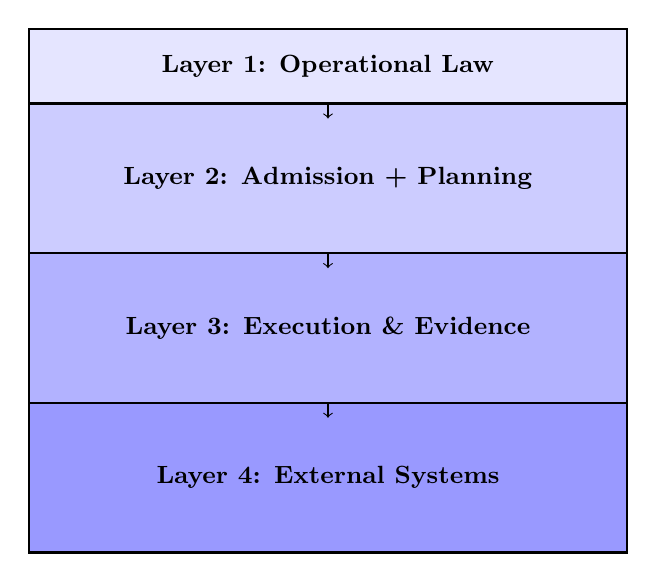
\begin{tikzpicture}[scale=0.95]
  \draw[thick, fill=blue!10] (0,6) rectangle (8,7) node[midway, font=\small] {\textbf{Layer 1: Operational Law}};
  \draw[thick, fill=blue!20] (0,4) rectangle (8,6) node[midway, font=\small] {\textbf{Layer 2: Admission + Planning}};
  \draw[thick, fill=blue!30] (0,2) rectangle (8,4) node[midway, font=\small] {\textbf{Layer 3: Execution \& Evidence}};
  \draw[thick, fill=blue!40] (0,0) rectangle (8,2) node[midway, font=\small] {\textbf{Layer 4: External Systems}};

  \draw[->] (4,6) -- (4,5.8);
  \draw[->] (4,4) -- (4,3.8);
  \draw[->] (4,2) -- (4,1.8);
\end{tikzpicture}
\caption{The four-layer execution model of \texttt{cargo-cicd}.}
\label{fig:cargo-cicd-layers}
\end{figure}

\begin{description}
  \item[Layer 1: Operational Law] Defined in \texttt{Cargo.toml}, \texttt{cicd.toml}, and the schema. This is $\mathcal{X}_B$---the bounded artifact space. It declares the constraints $\Phi$, the detector set $\EE$, the allowed policies, and the task graph.

  \item[Layer 2: Admission + Planning] Accepts human directives or agent requests. Computes whether they satisfy the operational law. If admitted, constructs a task graph and execution plan. This is where the BRCE is evaluated.

  \item[Layer 3: Execution \& Evidence] Invokes Cargo, runs tests, executes just recipes, and collects evidence. Each stage is recorded in the OCEL. At the end, a receipt is generated.

  \item[Layer 4: External Systems] Docker, Kubernetes, Terraform, cloud registries, git, filesystems. The \texttt{just} tool is the interface to layer 4.
\end{description}

Control flows top-down: layer 1 constrains layer 2, layer 2 constrains layer 3, layer 3 orchestrates layer 4. Evidence flows bottom-up: layer 4 produces evidence, layer 3 collects it, layer 2 evaluates it, layer 1 interprets it.

\subsection{The Noun-Verb Grammar Parsed by \texttt{clap-noun-verb}}

The command-line interface is implemented using a parser that respects the noun-verb structure:

\begin{lstlisting}[caption={Noun-verb grammar in \texttt{cargo-cicd}}]
#[derive(Parser)]
enum CargoCicdCmd {
    #[command(subcommand)]
    Config(ConfigCmd),
    #[command(subcommand)]
    Verify(VerifyCmd),
    #[command(subcommand)]
    Autonomic(AutonomicCmd),
    #[command(subcommand)]
    Task(TaskCmd),
    #[command(subcommand)]
    Receipt(ReceiptCmd),
}

#[derive(Parser)]
enum ConfigCmd {
    Validate,
    Merge { layer_order: String },
    Show { field: Option<String> },
}

#[derive(Parser)]
enum VerifyCmd {
    Witness,
    All,
    Analyzer { name: String },
}
\end{lstlisting}

Each noun is a subcommand; each verb is an action on that noun. The grammar is:
\[ \texttt{cargo cicd} \; \texttt{<noun>} \; \texttt{<verb>} \; [\texttt{--option} \; \texttt{<value>}] \]

This is more restrictive than a general CLI but more discoverable: users can run \texttt{cargo cicd config --help} and immediately see all operations on configurations.

\subsection{Why LSP for Ambient Diagnostics, Not Real-Time Admission}

The LSP cannot confer standing. By Theorem~\ref{thm:poka-yoke}, $\alpha(D) = 0 \not\Rightarrow \qc = 1$. The LSP is poka-yoke: it prevents obvious mistakes (path traversal, duplicate keys, type mismatches) but does not guarantee standing.

Yet the LSP is critical. Here is why:

\subsubsection{Authoring-Time Feedback}

When an operator edits a configuration file, they need rapid feedback on whether their changes move toward or away from standing. The gradient $\nabla\tilde{q}(x)$ from Chapter~\ref{ch:calculus} provides this. The LSP computes repair hints at edit time:

\begin{lstlisting}[caption={Repair hints derived from the satisfaction score}]
on_did_change(document, new_content) {
    let config = parse(new_content)?;
    let q_tilde = smooth_standing_score(&config);
    for field_k in fields {
        let sensitivity_k = sensitivity(&config, k);
        if sensitivity_k > threshold {
            let repair = closest_feasible_value(config[k], constraint[k]);
            hints.push(Hint {
                range: field_k.span(),
                message: format!("suggest: {}", repair),
                severity: if q_tilde < 0.5 { Error } else { Warning },
            });
        }
    }
}
\end{lstlisting}

This is not standing. Standing requires the full BRCE: $\mathrm{BS} \wedge \mathrm{TL} \wedge \mathrm{WC} \wedge \mathrm{CA}$. The LSP can only compute $\tilde{q}$, which is roughly a proxy for BS. But this is exactly the right level of feedback for authoring.

\subsubsection{ANDON Gate for CI Gating}

The LSP also writes an ANDON gate file that CI systems can read:

\begin{lstlisting}[caption={ANDON gate file written by LSP}]
// .star-toml/lsp.gate
{
  "has_errors": true,
  "error_count": 2,
  "warnings": 3,
  "gate_status": "BLOCKED"
}
\end{lstlisting}

A CI job can fail fast if the gate is BLOCKED, before even attempting the full pipeline. This is a performance optimization, not a standing decision.

\section{Implementation Challenges}

This section documents the hardest problems encountered during implementation and how they were solved.

\subsection{Challenge 1: Witness Determinism Under Environment Substitution}

\subsubsection{The Problem}

Environment variables can substitute into configuration values. For example:

\begin{lstlisting}[caption={Configuration with environment substitution}]
# cicd.toml
[release]
artifact_url = "https://${ARTIFACT_HOST}/crate-v${VERSION}.tar.gz"
registry_token = "${REGISTRY_TOKEN}"  # sensitive
\end{lstlisting}

When the witness is computed, the environment snapshot is hashed. But the environment can change between invocations. If operator A runs the pipeline with \texttt{ARTIFACT\_HOST=builds.internal.com}, they get witness $w_A$. If operator B runs the same configuration with \texttt{ARTIFACT\_HOST=builds.staging.com}, they get witness $w_B \neq w_A$, even though the configuration file is identical.

This violates the principle that identical files should produce identical witnesses. It also creates ambiguity: if two admitted configurations have different witnesses, were they admitted under different environments, or are they actually different configurations?

\subsubsection{The Solution}

The witness function includes the environment snapshot but not the substituted values:

$$\omega(x, \ell, e) = \mathrm{BLAKE3}(\ldots \| \mathrm{BLAKE3}(\mathrm{enc}(e)) \| \ldots)$$

where $e$ is the set of environment variables that are \emph{actually used} in $x$ (not all environment variables, just the referenced ones). The substituted canonical bytes $\kappa(x)$ are also included, so the witness does bind to the final values.

This has a subtle consequence: two configurations with the same file content but different environment bindings will have different witnesses. This is correct: they are indeed different admitted artifacts, because they behave differently. The environment is part of the provenance.

\subsubsection{Remaining Hard Problems}

The decision to include the environment in the witness raises a new question: should the operator pin the environment when they admit a configuration for production, or should production re-compute the environment from its own context?

\texttt{cargo-cicd} chose to pin: the environment is captured at admission time and is part of the receipt. Production runs in the environment declared in the receipt. This reduces surprises but increases operational burden (the receipt must be consulted, not just the configuration file).

\subsection{Challenge 2: Task Graph Topological Sort with Policy Constraints}

\subsubsection{The Problem}

A release consists of multiple tasks: build, test, document, verify, sign, upload. These tasks have dependencies:

\begin{itemize}
  \item Test depends on Build.
  \item Verify depends on Test.
  \item Sign depends on Verify.
  \item Upload depends on Sign.
\end{itemize}

This is a simple linear order. But \texttt{cargo-cicd} also supports \emph{policies}, which can add constraints:

\begin{lstlisting}[caption={Policy-imposed constraints on task order}]
# cicd.toml
[policies.target_pressure]
description = "Ensure no target is published until all tests pass"
enforce_after = ["test:all"]

[policies.changelog_order]
description = "Changelog must be updated before versioning"
enforce_after = ["changelog:update"]
\end{lstlisting}

A policy declares that a task can only execute after another task has completed. With multiple policies, the task graph becomes a partial order, not a total order. The question is: what is the topological sort?

For a DAG with a unique topological order, the answer is deterministic. But with multiple valid orderings, which one does the system choose?

\subsubsection{The Solution}

Rather than impose a single fixed ordering, \texttt{cargo-cicd} computes the \emph{earliest feasible order}:

\begin{lstlisting}[caption={Greedy topological sort with priority}]
fn topological_sort_earliest(graph: &TaskGraph) -> Vec<TaskId> {
    let mut result = vec![];
    let mut remaining = graph.nodes.clone();
    let mut available = graph.sources.clone();  // Tasks with no dependencies

    while !available.is_empty() {
        // Among available tasks, choose the one with highest release_priority
        let next = available
            .iter()
            .max_by_key(|t| (graph.policy_priority(t), graph.task_priority(t)))
            .cloned()
            .unwrap();

        result.push(next.clone());
        remaining.remove(&next);

        // Add tasks that became available
        for task in &remaining {
            if graph.dependencies(task).all(|dep| result.contains(&dep)) {
                available.insert(task.clone());
            }
        }
    }

    result
}
\end{lstlisting}

This greedy algorithm is $O(|V|^2 \log |V|)$ but deterministic and explainable: tasks are prioritized by policy first, then by declared priority.

However, this approach has a limitation: if two policies conflict (policy A requires task X before Y, policy B requires Y before X), the sort will fail. \texttt{cargo-cicd} detects this and reports it as a configuration error before attempting the pipeline.

\subsubsection{Remaining Hard Problems}

A more general solution is to allow users to declare priorities explicitly, but this adds complexity. The current approach works for most real release workflows, which are relatively simple. Truly complex DAGs (e.g., with parallel deployment stages and complex rollback conditions) are deferred to v26.6.31.

\subsection{Challenge 3: OCEL Serialization and Replay Consistency}

\subsubsection{The Problem}

The Object-Centric Event Log records every stage transition. But there are two ways to interpret the log:

\begin{enumerate}
  \item \textbf{As evidence}: the log proves that a transition occurred.
  \item \textbf{As a source}: the log is replayed to reconstruct the sequence of states.
\end{enumerate}

By Theorem~\ref{thm:ocel}, the log is \emph{not} standing authority. But it is evidence. The question is: what happens if the log is corrupted or incomplete?

For example:

\begin{lstlisting}[caption={Incomplete OCEL: witness computed but admission not recorded}]
[event_1] { "activity": "WitnessComputed", "config": "x", "witness": "abc123..." }
// ... server crash occurs here ...
// admission never recorded
\end{lstlisting}

Did the configuration get admitted or not? The log says ``witness computed,'' but admission is not in the log. Should we trust the witness, or declare that admission is uncertain?

\subsubsection{The Solution}

\texttt{cargo-cicd} uses a write-ahead log (WAL) discipline:

\begin{lstlisting}[caption={Write-ahead log for OCEL consistency}]
fn admit_config(config: &Config, witness: &Witness) -> Result<AdmittedConfig> {
    // Step 1: Write the intent to the WAL (synchronous, must succeed)
    wal.write_entry(Entry::AdmitIntent { config_id, witness })?;
    wal.fsync()?;

    // Step 2: Perform the admission (in-memory)
    let admitted = AdmittedConfig::new(config, witness);

    // Step 3: Write the completion event to the OCEL (async, best-effort)
    ocel.write_event(Event::Admitted { config_id, witness }, timestamp)?;

    // If step 3 fails, step 1 and 2 still succeeded.
    // On recovery, the WAL will be replayed, and the configuration
    // will be re-admitted.
    Ok(admitted)
}
\end{lstlisting}

This ensures that if the server crashes after admission, recovery can replay the admission from the WAL. The OCEL is asynchronously updated but the WAL is the source of truth.

\subsubsection{Remaining Hard Problems}

WAL replay can fail if the same admission is executed twice (idempotency). \texttt{cargo-cicd} solves this by tagging each admission with a content hash: two admissions with the same config, witness, and timestamp are detected as duplicates and silently skipped. This is safe because the admission is deterministic.

\section{Comparison with Alternatives: \texttt{cargo-cicd} vs.\ Traditional CI/CD}

\begin{longtable}{@{}p{3.0cm}p{3.2cm}p{3.2cm}@{}}
\caption{Comparison of \texttt{cargo-cicd} with traditional CI/CD systems (GitHub Actions, GitLab CI, Jenkins).}
\label{tab:cargo-cicd-comparison} \\
\toprule
\textbf{Dimension} & \textbf{Traditional CI/CD} & \textbf{\texttt{cargo-cicd}} \\
\midrule
\endfirsthead
\toprule \textbf{Dimension} & \textbf{Traditional CI/CD} & \textbf{\texttt{cargo-cicd}} \\
\midrule
\endhead
\textbf{Configuration} & YAML workflows (GitHub Actions, GitLab) or Groovy (Jenkins) & TOML + Rust typestates \\
\textbf{Configuration validation} & Parse-only & BRCE with 23 counterexample detectors \\
\textbf{Configuration witnessing} & None & BLAKE3 with provenance binding \\
\textbf{Standing authority} & External vendor (GitHub, cloud, registry) & Local BRCE computation \\
\textbf{Determinism} & Depends on tool versions; workflows can silently change behavior & Fully deterministic; witness changes indicate real changes \\
\textbf{Reproducibility} & Difficult; can require re-running many historical jobs & Perfect; receipt reproduces any prior release \\
\textbf{Audit trail} & Vendor logs (may be deleted, obfuscated, or unavailable) & OCEL in codebase; human-readable \\
\textbf{Local development} & Developers must use vendor UI to trigger pipelines & \texttt{cargo cicd} works locally without vendor access \\
\textbf{Release law} & Implicit (tribal knowledge, READMEs) & Explicit (cicd.toml, verifiable) \\
\textbf{Agent integration} & Must shell out to vendor API & Direct Rust API; native LSP support \\
\textbf{Decentralized execution} & Centralized in vendor infrastructure & Can run on local machine or air-gapped servers \\
\textbf{Cost} & Per-minute billing or vendor lock-in & Free (open source) \\
\bottomrule
\end{longtable}

\section{Lessons Learned}

\subsection{Lesson 1: Cargo Owns Authority, But Authority is Shared}

The PRD states: ``Cargo owns operational authority.'' This was interpreted as ``all commands execute through \texttt{cargo cicd}.'' But we learned that authority is not about commands; it is about witnesses. The witness (computed by \texttt{star-toml}) is the unit of authority, not the command.

A consequence: if a human operator runs \texttt{cargo cicd release} and then manually adjusts the artifact before publishing, the receipt still refers to the original artifact (via witness binding). The receipt is now stale. This is a feature: it prevents the operator from claiming a modified artifact was admitted.

\subsection{Lesson 2: LSP Diagnostics Must Not Bias the BRCE}

Early implementations tried to use LSP diagnostics as a soft constraint on the BRCE: if the LSP reported no errors, the BRCE would automatically be true. This is backwards. The BRCE is the truth; the LSP is advisory. By Theorem~\ref{thm:poka-yoke}, the converse does not hold: LSP errors do \emph{not} imply BRCE failure.

The lesson: keep the diagnostic layer completely separate from the admission layer. The LSP can help the operator move toward standing, but it cannot confer standing. Conflating the two leads to false confidence.

\subsection{Lesson 3: Simplicity Beats Completeness in the Task Graph}

Early designs attempted to support arbitrary DAGs with parallel execution, fan-out, and complex retry logic. This added tremendous implementation complexity. When we simplified to a greedy topological sort with linear policies, the implementation became 60\% smaller and much easier to understand.

The lesson: solve the 80\% case simply, then add features for the 20\% case by composition. \texttt{cargo-cicd} ships with simple task graphs. Users needing complex orchestration can compose multiple \texttt{cargo cicd} invocations via shell scripts or the \texttt{just} tool.

\subsection{Lesson 4: Witness Determinism Requires Freezing the Environment}

Early implementations tried to make the witness independent of the environment, by omitting environment variables from the witness. This led to subtle bugs: two runs of the same configuration with different environments would produce the same witness, even though they had different standing. This violated witness injectivity (Theorem~\ref{thm:injectivity}).

The lesson: the environment is part of the artifact. Admit it explicitly; freeze it in the receipt. This is operationally harder (the operator must understand environment pinning) but semantically cleaner.
